\begin{problem}{스타링크 노래 맞히기}{standard input}{standard output}{1 second}{256 megabytes}

윤수는 스타링크 노래 맞히기를 좋아한다. 스타링크 노래 맞히기는 주어진 노래를 듣고 먼저 제목을 맞히는 사람이 점수를 얻는 게임이다. 절대 음감을 가진 윤수는 노래의 첫 네 음만 듣고도 어떤 노래든 바로 맞출 수 있다. 정환은 윤수랑 맞서 싸울 수 있는 프로그램을 만들려고 한다. 다음은 TwinkleTwinkleLittleStar(반짝반짝 작은 별)의 악보 중 일부이다.
\begin{center}
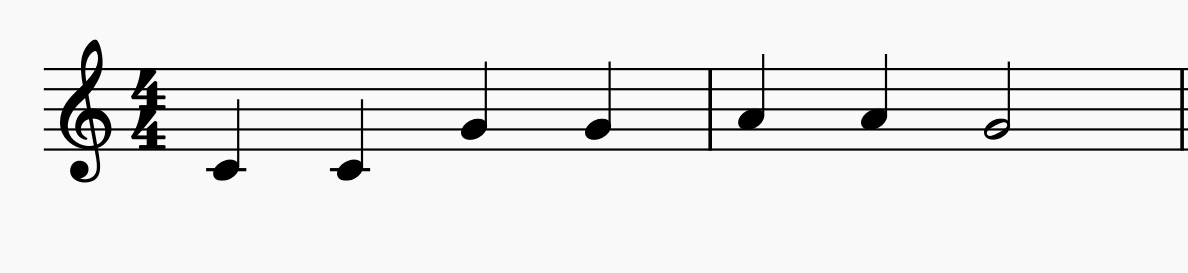
\includegraphics[bb=0 0 100 200]{starlink.png}
\end{center} 

악보를 박자와 관계없이 음이름으로 표현하면 다음과 같다. "CCGGAAG"[도도솔솔라라솔]

윤수를 이기기 위해서는 이 프로그램이 첫 세 음인 CCG만 듣고 노래 제목인 TwinkleTwinkleLittleStar를 출력할 수 있어야 한다. 세상의 모든 노래를 아는 윤수와 다르게 정환은 음을 아는 노래가 $N$개 뿐이다. 만약 노래의 첫 음 3개로 시작하는 노래가 여러개 있어 무슨 노래인지 알 수 없는 경우 \t{?}를 출력한다. 또한, 정환이 알지 못하는 노래가 나올 경우 \t{!}를 출력한다.

정환을 도와서 첫 세 음만 듣고 본인이 음을 아는 노래를 맞추는 프로그램을 완성시키자. 이 프로그램은 대문자와 소문자를 구분한다.

\InputFile
첫째 줄에는 정환이 음을 아는 노래의 개수 $N(1 ≤ N ≤ 1,000)$개 질문의 개수 $M(1 ≤ M ≤ 1000)$개가 공백으로 구분되어 들어온다.

둘째 줄부터 $N$개의 줄에는 노래 제목의 길이 $T(1 ≤ T ≤ 30)$, 영어 대소문자로 이루어진 노래 제목 $S$, 해당 노래의 첫 일곱 음이름 $a_1, a_2, a_3, a_4, a_5, a_6, a_7$이 공백으로 구분되어 주어진다. 음이름의 경우에 $A, B, C, D, E, F, G$ 7개로 만 구성 되어있다. 노래 제목의 경우에 동일한 제목이 주어지지 않는다.

$N+2$번째 줄 부터 $M$개줄 동안에는 음이름 $b_1, b_2, b_3$가 빈칸으로 분리되어 들어온다.

\OutputFile
주어지는 질문 순서대로 첫 세 음과 동일한 노래가 정확하게 하나 있다면 해당 노래의 제목을, 첫 세 음과 동일한 노래가 두 개 이상이면 \t{?}을, 첫 세 음과 동일한 노래가 없다면 \t{!}을 한 줄에 하나씩 출력한다.

\Example

\begin{example}
\exmpfile{example.01}{example.01.a}%
\end{example}

\end{problem}

